%%%%%%%%%%%%%%%%%%%%%%%%%%%%%%%%%%%%%%%%%%%%%%%%%%%%%%%%%%%%%%%
%
% Welcome to Overleaf --- just edit your LaTeX on the left,
% and we'll compile it for you on the right. If you open the
% 'Share' menu, you can invite other users to edit at the same
% time. See www.overleaf.com/learn for more info. Enjoy!
%
%%%%%%%%%%%%%%%%%%%%%%%%%%%%%%%%%%%%%%%%%%%%%%%%%%%%%%%%%%%%%%%


% Inbuilt themes in beamer
\documentclass{beamer}
\usepackage{setspace}
\usepackage{gensymb}
\singlespacing
\usepackage{amsmath}
\usepackage{bm}
\usepackage{cite}
\usepackage{cases}
\usepackage{subfig}
\usepackage{longtable}
\usepackage{multirow}
\usepackage{verbatim}
\usepackage{hyperref}
\usepackage{listings}
\usepackage{color}    
\usepackage{array}    
\usepackage{longtable}
\usepackage{calc}     
\usepackage{multirow} 
\usepackage{hhline}   
\usepackage{ifthen}   
\DeclareMathOperator*{\Res}{Res}

% correct bad hyphenation here
\hyphenation{op-tical net-works semi-conduc-tor}
\def\inputGnumericTable{}                                 %%

\lstset{
%language=C,
frame=single, 
breaklines=true,
columns=fullflexible
}
%\lstset{
%language=tex,
%frame=single, 
%breaklines=true
%}
\hypersetup{
    colorlinks=true,
    linkcolor=black,
    urlcolor=blue,
}
\usetheme{CambridgeUS}

\DeclareMathOperator*{\argmax}{arg\,max}
\DeclareMathOperator*{\argmin}{arg\,min}
\newtheorem{proposition}{Proposition}[section]
\newcommand{\BEQA}{\begin{eqnarray}}
\newcommand{\EEQA}{\end{eqnarray}}
\newcommand{\define}{\stackrel{\triangle}{=}}
\bibliographystyle{IEEEtran}
\providecommand{\mbf}{\mathbf}
\providecommand{\pr}[1]{\ensuremath{\Pr\left(#1\right)}}
\providecommand{\qfunc}[1]{\ensuremath{Q\left(#1\right)}}
\providecommand{\sbrak}[1]{\ensuremath{{}\left[#1\right]}}
\providecommand{\lsbrak}[1]{\ensuremath{{}\left[#1\right.}}
\providecommand{\rsbrak}[1]{\ensuremath{{}\left.#1\right]}}
\providecommand{\brak}[1]{\ensuremath{\left(#1\right)}}
\providecommand{\lbrak}[1]{\ensuremath{\left(#1\right.}}
\providecommand{\rbrak}[1]{\ensuremath{\left.#1\right)}}
\providecommand{\cbrak}[1]{\ensuremath{\left\{#1\right\}}}
\providecommand{\lcbrak}[1]{\ensuremath{\left\{#1\right.}}
\providecommand{\rcbrak}[1]{\ensuremath{\left.#1\right\}}}
\theoremstyle{remark}
\newtheorem{rem}{Remark}
\newcommand{\sgn}{\mathop{\mathrm{sgn}}}
\providecommand{\abs}[1]{\left\vert#1\right\vert}
\providecommand{\res}[1]{\Res\displaylimits_{#1}} 
\providecommand{\norm}[1]{\left\lVert#1\right\rVert}
\providecommand{\mtx}[1]{\mathbf{#1}}
\providecommand{\mean}[1]{\mathbb{E}\left[ #1 \right]}   
\providecommand{\fourier}{\overset{\mathcal{F}}{ \rightleftharpoons}}
\providecommand{\system}[1]{\overset{\mathcal{#1}}{ \longleftrightarrow}}
\newcommand{\cosec}{\,\text{cosec}\,}
\providecommand{\dec}[2]{\ensuremath{\overset{#1}{\underset{#2}{\gtrless}}}}
\newcommand{\myvec}[1]{\ensuremath{\begin{pmatrix}#1\end{pmatrix}}}
\newcommand{\mydet}[1]{\ensuremath{\begin{vmatrix}#1\end{vmatrix}}}
\renewcommand{\vec}[1]{\mathbf{\boldsymbol{#1}}}
% Theme choice:
\newcounter{saveenumi}
\newcommand{\seti}{\setcounter{saveenumi}{\value{enumi}}}
\newcommand{\conti}{\setcounter{enumi}{\value{saveenumi}}}

\resetcounteronoverlays{saveenumi}
% Title page details: 
\title[Machine Learning for Student Evaluation]{An Application of Machine Learning to Grading} 
\author{Gautam Singh}
\begin{document}

% Title page frame
\begin{frame}
    \titlepage 
\end{frame}

% Remove logo from the next slides
\logo{}

% Outline frame
\begin{frame}{Outline}
    \tableofcontents
\end{frame}


% Lists frame
\section{Introduction}
\begin{frame}{Aim}
    Compare grade distribution obtained by using the $K$-means algorithm to 
    the grade distribution obtained using a standard normal distribution.
    \pause
    \begin{enumerate}
        \item Which method is fairer?
        \pause
        \begin{enumerate}
            \item For courses with skewed performance?
            \pause
            \item For courses with less students :)?
        \end{enumerate}
        \pause
        \item Which method is faster to compute grades?
        \pause
        \item Which method reflects student efforts better? What about failing 
        students?
        \pause
        \item Which method can be extended to assess based on other factors?
    \end{enumerate}
\end{frame}

\section{Resources}
\begin{frame}{Resources}
Marks datasheet and relevant Python codes can be found 
\href{https://github.com/goats-9/ee2802-assignments/tree/main/grading/codes}{here}.
\begin{enumerate}
    \item Marks of students: \texttt{marks.xlsx}
    \item Python code using Gaussian method: \texttt{grades\_norm.py}
    \item Python code using $K$-means method: \texttt{grades.py}
\end{enumerate}
\end{frame}

\begin{frame}{Data Visualization}
    \pause
    \begin{figure}[!ht]
        \centering
        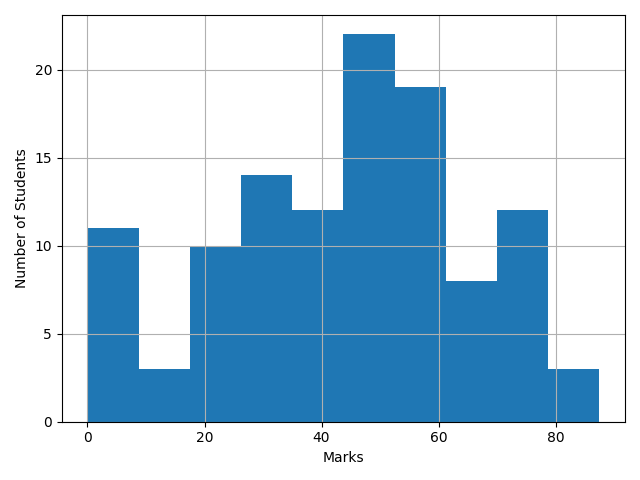
\includegraphics[width=0.6\columnwidth]{figs/dataset.png}
        \caption{Histogram showing distribution of marks of the students.}
        \label{fig:data}
    \end{figure}
\end{frame}

\section{Grading Using the Gaussian Method}

\begin{frame}{Population Measures}
    Consider a dataset $\cbrak{\vec{x}_i}_{i=1}^N$.
    \pause
    \begin{enumerate}
        \item The \textbf{population mean} is given by
            \begin{align}
                \vec{\mu} &\triangleq \mean{\vec{x}}
                \label{eq:mean}
            \end{align}
        \pause
        \item The \textbf{population covariance matrix} is given by
            \begin{align}
                \vec{\Sigma} &\triangleq \mean{\brak{\vec{x}-\vec{\mu}}\brak{\vec{x}-\vec{\mu}}^\top}
                \label{eq:var}
            \end{align}
    \end{enumerate}
\end{frame}

\begin{frame}{Sample Measures}
    Consider a sample $\cbrak{\vec{y}_i}_{i=1}^n$ drawn from the earlier dataset 
    ($n \ll N$).
    \pause
    \begin{enumerate}
        \item The \textbf{sample mean} is given by
            \begin{align}
                \bar{\vec{x}} &\triangleq \mean{\vec{y}}
                \label{eq:smpl-mean}
            \end{align}
        \pause
        \item The \textbf{sample covariance matrix} is given by
            \begin{align}
                \vec{s} &\triangleq \frac{n}{n-1} \mean{\brak{\vec{y}-\bar{\vec{x}}}\brak{\vec{x}-\bar{\vec{x}}}^\top}
                \label{eq:smpl-var}
            \end{align}
        \pause
    \end{enumerate}
    Note that the sample measures are \textbf{unbiased estimators} of their
    corresponding population measures.
\end{frame}

\begin{frame}{The $Z$-score}
    \pause
    \begin{enumerate}
        \item We assume that the number of students is large and the distribution
        of their parameters follows a normal distribution with population mean 
        $\vec{\mu}$ and population covariance $\vec{\Sigma}$.
        \pause
        \item The $Z$-score of a student given their parameters $\vec{x}$ is 
        given by
        \begin{align}
            \vec{Z} \triangleq \vec{\Sigma}^{-\frac{1}{2}}\brak{\vec{x}-\vec{\mu}}
            \label{eq:Z-score}
        \end{align}
        \pause
    \end{enumerate}
    \begin{alertblock}{Statistical Note}
        If the population is large, computing population parameters directly
        is cumbersome. In this case, use the sample parameters to calculate
        the $Z$-score.
    \end{alertblock}
\end{frame}

\begin{frame}{Application}
    In this case, data is one dimensional (marks of the student). Also, the
    population size is small enough to directly compute population measures.
    \pause
    \begin{enumerate}
        \item The $Z$-score in this case will be
            \begin{align}
                Z = \frac{x-\mu}{\sigma}
                \label{eq:Z-score-app}
            \end{align}
        where $x$ denotes the marks of the student.
        \pause
        \item The runtime in this case is $O\brak{N}$.
        \pause
        \item The marks were scaled relative to the highest scoring student.
    \end{enumerate}
\end{frame}

\begin{frame}{Grading Scheme}
    \pause
    \begin{table}[!ht]
        \centering
        %%%%%%%%%%%%%%%%%%%%%%%%%%%%%%%%%%%%%%%%%%%%%%%%%%%%%%%%%%%%%%%%%%%%%%
%%                                                                  %%
%%  This is the header of a LaTeX2e file exported from Gnumeric.    %%
%%                                                                  %%
%%  This file can be compiled as it stands or included in another   %%
%%  LaTeX document. The table is based on the longtable package so  %%
%%  the longtable options (headers, footers...) can be set in the   %%
%%  preamble section below (see PRAMBLE).                           %%
%%                                                                  %%
%%  To include the file in another, the following two lines must be %%
%%  in the including file:                                          %%
%%        \def\inputGnumericTable{}                                 %%
%%  at the beginning of the file and:                               %%
%%        \input{name-of-this-file.tex}                             %%
%%  where the table is to be placed. Note also that the including   %%
%%  file must use the following packages for the table to be        %%
%%  rendered correctly:                                             %%
%%    \usepackage[latin1]{inputenc}                                 %%
%%    \usepackage{color}                                            %%
%%    \usepackage{array}                                            %%
%%    \usepackage{longtable}                                        %%
%%    \usepackage{calc}                                             %%
%%    \usepackage{multirow}                                         %%
%%    \usepackage{hhline}                                           %%
%%    \usepackage{ifthen}                                           %%
%%  optionally (for landscape tables embedded in another document): %%
%%    \usepackage{lscape}                                           %%
%%                                                                  %%
%%%%%%%%%%%%%%%%%%%%%%%%%%%%%%%%%%%%%%%%%%%%%%%%%%%%%%%%%%%%%%%%%%%%%%



%%  This section checks if we are begin input into another file or  %%
%%  the file will be compiled alone. First use a macro taken from   %%
%%  the TeXbook ex 7.7 (suggestion of Han-Wen Nienhuys).            %%
\def\ifundefined#1{\expandafter\ifx\csname#1\endcsname\relax}


%%  Check for the \def token for inputed files. If it is not        %%
%%  defined, the file will be processed as a standalone and the     %%
%%  preamble will be used.                                          %%
\ifundefined{inputGnumericTable}

%%  We must be able to close or not the document at the end.        %%
	\def\gnumericTableEnd{\end{document}}


%%%%%%%%%%%%%%%%%%%%%%%%%%%%%%%%%%%%%%%%%%%%%%%%%%%%%%%%%%%%%%%%%%%%%%
%%                                                                  %%
%%  This is the PREAMBLE. Change these values to get the right      %%
%%  paper size and other niceties.                                  %%
%%                                                                  %%
%%%%%%%%%%%%%%%%%%%%%%%%%%%%%%%%%%%%%%%%%%%%%%%%%%%%%%%%%%%%%%%%%%%%%%

	\documentclass[12pt%
			  %,landscape%
                    ]{report}
       \usepackage[latin1]{inputenc}
       \usepackage{fullpage}
       \usepackage{color}
       \usepackage{array}
       \usepackage{longtable}
       \usepackage{calc}
       \usepackage{multirow}
       \usepackage{hhline}
       \usepackage{ifthen}

	\begin{document}


%%  End of the preamble for the standalone. The next section is for %%
%%  documents which are included into other LaTeX2e files.          %%
\else

%%  We are not a stand alone document. For a regular table, we will %%
%%  have no preamble and only define the closing to mean nothing.   %%
    \def\gnumericTableEnd{}

%%  If we want landscape mode in an embedded document, comment out  %%
%%  the line above and uncomment the two below. The table will      %%
%%  begin on a new page and run in landscape mode.                  %%
%       \def\gnumericTableEnd{\end{landscape}}
%       \begin{landscape}


%%  End of the else clause for this file being \input.              %%
\fi

%%%%%%%%%%%%%%%%%%%%%%%%%%%%%%%%%%%%%%%%%%%%%%%%%%%%%%%%%%%%%%%%%%%%%%
%%                                                                  %%
%%  The rest is the gnumeric table, except for the closing          %%
%%  statement. Changes below will alter the table's appearance.     %%
%%                                                                  %%
%%%%%%%%%%%%%%%%%%%%%%%%%%%%%%%%%%%%%%%%%%%%%%%%%%%%%%%%%%%%%%%%%%%%%%

\providecommand{\gnumericmathit}[1]{#1} 
%%  Uncomment the next line if you would like your numbers to be in %%
%%  italics if they are italizised in the gnumeric table.           %%
%\renewcommand{\gnumericmathit}[1]{\mathit{#1}}
\providecommand{\gnumericPB}[1]%
{\let\gnumericTemp=\\#1\let\\=\gnumericTemp\hspace{0pt}}
 \ifundefined{gnumericTableWidthDefined}
        \newlength{\gnumericTableWidth}
        \newlength{\gnumericTableWidthComplete}
        \newlength{\gnumericMultiRowLength}
        \global\def\gnumericTableWidthDefined{}
 \fi
%% The following setting protects this code from babel shorthands.  %%
 \ifthenelse{\isundefined{\languageshorthands}}{}{\languageshorthands{english}}
%%  The default table format retains the relative column widths of  %%
%%  gnumeric. They can easily be changed to c, r or l. In that case %%
%%  you may want to comment out the next line and uncomment the one %%
%%  thereafter                                                      %%
\providecommand\gnumbox{\makebox[0pt]}
%%\providecommand\gnumbox[1][]{\makebox}

%% to adjust positions in multirow situations                       %%
\setlength{\bigstrutjot}{\jot}
\setlength{\extrarowheight}{\doublerulesep}

%%  The \setlongtables command keeps column widths the same across  %%
%%  pages. Simply comment out next line for varying column widths.  %%
\setlongtables

\setlength\gnumericTableWidth{%
	53pt+%
	53pt+%
0pt}
\def\gumericNumCols{2}
\setlength\gnumericTableWidthComplete{\gnumericTableWidth+%
         \tabcolsep*\gumericNumCols*2+\arrayrulewidth*\gumericNumCols}
\ifthenelse{\lengthtest{\gnumericTableWidthComplete > \linewidth}}%
         {\def\gnumericScale{\ratio{\linewidth-%
                        \tabcolsep*\gumericNumCols*2-%
                        \arrayrulewidth*\gumericNumCols}%
{\gnumericTableWidth}}}%
{\def\gnumericScale{1}}

%%%%%%%%%%%%%%%%%%%%%%%%%%%%%%%%%%%%%%%%%%%%%%%%%%%%%%%%%%%%%%%%%%%%%%
%%                                                                  %%
%% The following are the widths of the various columns. We are      %%
%% defining them here because then they are easier to change.       %%
%% Depending on the cell formats we may use them more than once.    %%
%%                                                                  %%
%%%%%%%%%%%%%%%%%%%%%%%%%%%%%%%%%%%%%%%%%%%%%%%%%%%%%%%%%%%%%%%%%%%%%%

\ifthenelse{\isundefined{\gnumericColA}}{\newlength{\gnumericColA}}{}\settowidth{\gnumericColA}{\begin{tabular}{@{}p{53pt*\gnumericScale}@{}}x\end{tabular}}
\ifthenelse{\isundefined{\gnumericColB}}{\newlength{\gnumericColB}}{}\settowidth{\gnumericColB}{\begin{tabular}{@{}p{53pt*\gnumericScale}@{}}x\end{tabular}}

\begin{tabular}[c]{%
	b{\gnumericColA}%
	b{\gnumericColB}%
	}

%%%%%%%%%%%%%%%%%%%%%%%%%%%%%%%%%%%%%%%%%%%%%%%%%%%%%%%%%%%%%%%%%%%%%%
%%  The longtable options. (Caption, headers... see Goosens, p.124) %%
%	\caption{The Table Caption.}             \\	%
% \hline	% Across the top of the table.
%%  The rest of these options are table rows which are placed on    %%
%%  the first, last or every page. Use \multicolumn if you want.    %%

%%  Header for the first page.                                      %%
%	\multicolumn{2}{c}{The First Header} \\ \hline 
%	\multicolumn{1}{c}{colTag}	%Column 1
%	&\multicolumn{1}{c}{colTag}	\\ \hline %Last column
%	\endfirsthead

%%  The running header definition.                                  %%
%	\hline
%	\multicolumn{2}{l}{\ldots\small\slshape continued} \\ \hline
%	\multicolumn{1}{c}{colTag}	%Column 1
%	&\multicolumn{1}{c}{colTag}	\\ \hline %Last column
%	\endhead

%%  The running footer definition.                                  %%
%	\hline
%	\multicolumn{2}{r}{\small\slshape continued\ldots} \\
%	\endfoot

%%  The ending footer definition.                                   %%
%	\multicolumn{2}{c}{That's all folks} \\ \hline 
%	\endlastfoot
%%%%%%%%%%%%%%%%%%%%%%%%%%%%%%%%%%%%%%%%%%%%%%%%%%%%%%%%%%%%%%%%%%%%%%

\hhline{|-|-}
	 \multicolumn{1}{|p{\gnumericColA}|}%
	{\gnumericPB{\raggedright}\gnumbox[l]{\textbf{Interval}}}
	&\multicolumn{1}{p{\gnumericColB}|}%
	{\gnumericPB{\raggedright}\gnumbox[l]{\textbf{Grade}}}
\\
\hhline{|--|}
	 \multicolumn{1}{|p{\gnumericColA}|}%
	{\gnumericPB{\raggedright}\gnumbox[l]{($-\infty$, -3]}}
	&\multicolumn{1}{p{\gnumericColB}|}%
	{\gnumericPB{\raggedright}\gnumbox[l]{F}}
\\
\hhline{|--|}
	 \multicolumn{1}{|p{\gnumericColA}|}%
	{\gnumericPB{\raggedright}\gnumbox[l]{(-3, -2]}}
	&\multicolumn{1}{p{\gnumericColB}|}%
	{\gnumericPB{\raggedright}\gnumbox[l]{D}}
\\
\hhline{|--|}
	 \multicolumn{1}{|p{\gnumericColA}|}%
	{\gnumericPB{\raggedright}\gnumbox[l]{(-2, 1]}}
	&\multicolumn{1}{p{\gnumericColB}|}%
	{\gnumericPB{\raggedright}\gnumbox[l]{C}}
\\
\hhline{|--|}
	 \multicolumn{1}{|p{\gnumericColA}|}%
	{\gnumericPB{\raggedright}\gnumbox[l]{(-1, 0]}}
	&\multicolumn{1}{p{\gnumericColB}|}%
	{\gnumericPB{\raggedright}\gnumbox[l]{B-}}
\\
\hhline{|--|}
	 \multicolumn{1}{|p{\gnumericColA}|}%
	{\gnumericPB{\raggedright}\gnumbox[l]{(0, 1]}}
	&\multicolumn{1}{p{\gnumericColB}|}%
	{\gnumericPB{\raggedright}\gnumbox[l]{B}}
\\
\hhline{|--|}
	 \multicolumn{1}{|p{\gnumericColA}|}%
	{\gnumericPB{\raggedright}\gnumbox[l]{(1, 2]}}
	&\multicolumn{1}{p{\gnumericColB}|}%
	{\gnumericPB{\raggedright}\gnumbox[l]{A-}}
\\
\hhline{|--|}
	 \multicolumn{1}{|p{\gnumericColA}|}%
	{\gnumericPB{\raggedright}\gnumbox[l]{(2, 3]}}
	&\multicolumn{1}{p{\gnumericColB}|}%
	{\gnumericPB{\raggedright}\gnumbox[l]{A}}
\\
\hhline{|--|}
	 \multicolumn{1}{|p{\gnumericColA}|}%
	{\gnumericPB{\raggedright}\gnumbox[l]{(3,$\infty$)}}
	&\multicolumn{1}{p{\gnumericColB}|}%
	{\gnumericPB{\raggedright}\gnumbox[l]{A+}}
\\
\hhline{|-|-|}
\end{tabular}

\ifthenelse{\isundefined{\languageshorthands}}{}{\languageshorthands{\languagename}}
\gnumericTableEnd

        \caption{Grading scheme used for calculation of $Z$-scores}
        \label{tab:grade-scheme}
    \end{table}
\end{frame}

\section{Grading Using the K-Means Method}
\begin{frame}{The $K$-Means Algorithm}
    \pause
    \begin{enumerate}
        \item It is an \textbf{unsupervised} learning algorithm.
        \pause
        \item It is a \textbf{classification} algorithm.
        \pause
        \item It is an \textbf{EM} algorithm (explained ahead).
    \end{enumerate}
\end{frame}

\begin{frame}{Definitions}
    Consider a dataset $\cbrak{\vec{x}_n}_{n=1}^N$ and $K$ means
    $\cbrak{\vec{\mu}_k}_{k=1}^K$.
    \pause
    \begin{enumerate}
        \item We define \textbf{binary indicator variables} $r_{nk}$ for 
        $1 \le n \le N,\ 1 \le k \le K$ as
            \begin{align}
                r_{nk} \triangleq
                \begin{cases}
                    1 & k = \argmin_j\norm{\vec{x}_n-\vec{\mu}_j}^2 \\
                    0 & \textrm{otherwise}
                \end{cases}
                \label{eq:rnk-def}
            \end{align}
        \pause
        \item The \textbf{cost function} is given by
            \begin{align}
                J &\triangleq \sum_{n=1}^N\sum_{k=1}^Kr_{nk}\norm{\vec{x}_n-\vec{\mu}_{k}}^2
                \label{eq:cost-def}
            \end{align}
        \pause
        \item We are required to find $\cbrak{\vec{\mu}_k}_{k=1}^K$ such that
        \eqref{eq:cost-def} is \textit{minimized}.
    \end{enumerate}
\end{frame}

\begin{frame}{Working of the $K$-Means Algorithm}
    Initally, we choose an arbitrary set of means. In each iteration, there are 
    two steps.
    \pause
    \begin{enumerate}
        \item \textit{E-step}: Here, we calculate all the $r_{nk}$ as defined
            in \eqref{eq:rnk-def}.
        \pause
        \item \textit{M-step}: We set
            \begin{align}
                \vec{\mu}_k \leftarrow \frac{\sum_{n=1}^Nr_{nk}\vec{x}_n}{\sum_{n=1}^Nr_{nk}} = \frac{\vec{Xr}_k}{\vec{1}^\top\vec{r}_k}
                \label{eq:M-step}
            \end{align}
        \seti
    \end{enumerate}
\end{frame}

\begin{frame}{Working of the $K$-Means Algorithm (Contd...)}
    \begin{enumerate}
        \conti
        \item Here,
            \begin{align}
                \vec{X} &\triangleq \myvec{\vec{x}_1&\vec{x}_2&\ldots&\vec{x}_n} \\
                \vec{r}_k &\triangleq \myvec{r_{1k}&r_{2k}&\ldots&r_{nk}}^\top \\
                \vec{1} &\triangleq \myvec{1&1&\ldots&1}^\top
                \label{eq:M-defs}
            \end{align}
    \end{enumerate}
    \begin{alertblock}{What if a Cluster is Empty?}
        If we encounter a $k$ such that $\vec{r}_{k} = \vec{0}$, we can either
        \pause
        \begin{enumerate}
            \item Discard the cluster (by setting $K \leftarrow K - 1$)
            \pause
            \item Selecting a point ``far away'' from all clusters.
        \end{enumerate}
    \end{alertblock}
\end{frame}

\begin{frame}{Application}
    \pause
    \begin{enumerate}
        \item In this case, $K = 8$ and $N = 114$. The algorithm converged in 5 iterations.
        \pause
        \item The runtime in this case is $O\brak{NK}$ per iteration.
        \pause
        \item The marks were scaled relative to the highest scoring student.    
    \end{enumerate}
\end{frame}

\section{Results}
\begin{frame}
    \pause
    \begin{figure}
        \centering
        \subfloat[\centering Standard Normal Distribution]{{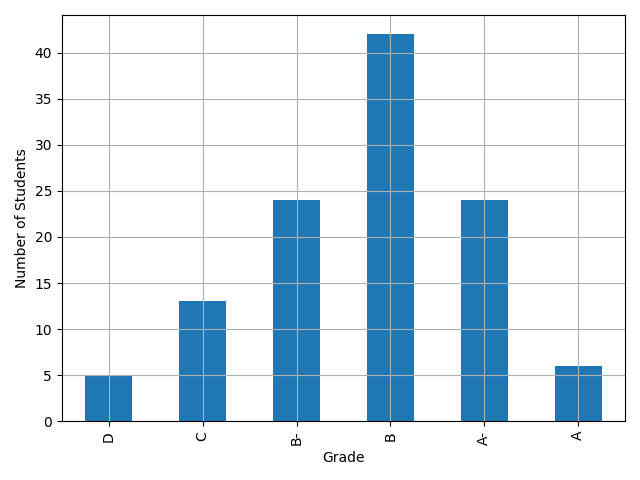
\includegraphics[width=0.45\columnwidth]{figs/grades_gauss.png}}}
        \qquad
        \subfloat[\centering $K$-Means Algorithm]{{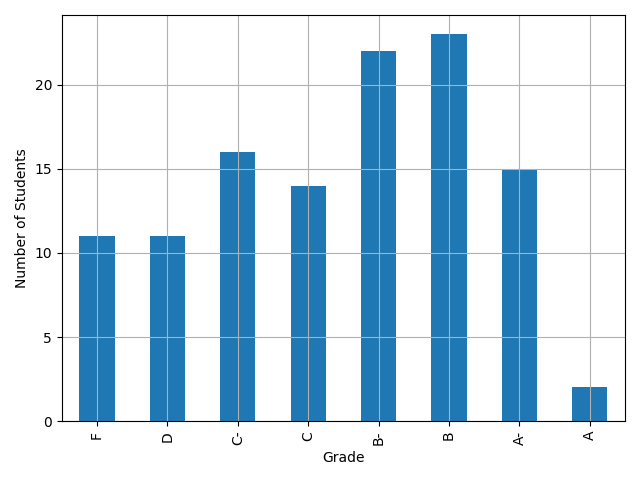
\includegraphics[width=0.45\columnwidth]{figs/grades_kmeans.png}}}
        \caption{Comparison of grading distributions using both algorithms.}
    \end{figure}
\end{frame}

\section{Conclusions}
\begin{frame}{Conclusions}
    \pause
    \begin{enumerate}
        \item Grading on a Gaussian curve failed less (in fact zero) students 
        than in the case of grading using the $K$-means algorithm.
        \pause
        \item Grading on a Gaussian curve is faster for larger datasets, and
        both algorithms would have very little difference.
        \pause
        \item The $K$-Means algorithm gives a better idea of the performance
        of the class, especially when it is skew.
        \pause
        \item The $K$-Means algorithm can be extended to involve other factors
        such as attendance, prerequisites completed, and so on.
    \end{enumerate}
\end{frame}
\end{document}
